\newpage
\subsection{Implementing check}
\texHeader
\hypertarget{checkCard tex}{}
 
\begin{itemize}
   
\item[$\blacktriangleright$] This time, we need to create three separate patterns - one to assert the guess, one to promote a card, and another to penalize.
Given that every action is determined with the result of a conditional, we need to create a proper control flow. We need an \emph{if/else} construct!

\item[$\blacktriangleright$] In the \texttt{check} declaration, create the basic \emph{if/else} construct with three patterns, as illustrated in
Fig.~\ref{fig:checkDec}.

\begin{figure}[htbp]
\begin{center}
  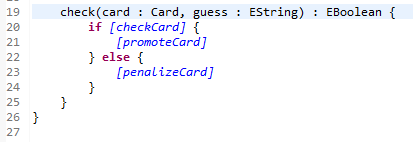
\includegraphics[width=0.65\textwidth]{eclipse_checkCardMethod}
  \caption{The \texttt{check} if/else construct}
  \label{fig:checkDec}
\end{center}
\end{figure} 

\item[$\blacktriangleright$] Upon saving, you should be immediately informed of 3 errors. Using the ``Quick Fix'' wizard, generate the pattern files for all
three. Your package explorer should now resemble Fig.~\ref{fig:checkPatternsExplorer}.

\begin{figure}[htbp]
\begin{center}
  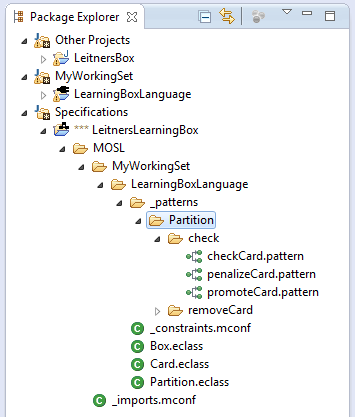
\includegraphics[width=0.55\textwidth]{eclipse_checkPackageExplorer}
  \caption{The created pattern files}
  \label{fig:checkPatternsExplorer}
\end{center}
\end{figure} 

\item[$\blacktriangleright$] Lets think about what we need in order to validate the guess. Given that \texttt{guess} is a parameter, the only object variable
we need to create in \texttt{checkCard.pattern} is a bounded \texttt{card}.

\item[$\blacktriangleright$] Now we need to compare the user's guess to the value on the back of the card. To do this, we need to specify an \emph{Attribute
Constraint}. Given that we created a \texttt{card} variable, we can access its value via a \texttt{card.back} statement. To access the paramter
value however, we need to preface the name in a '\$' operator. Finally, to complete the constraint, we need a comparison operator. Since we want them
to be the same, it would be a simple '==' command. Your rule should now resemble Fig.~\ref{fig:checkPattern}.

\begin{figure}[htbp]
\begin{center}
  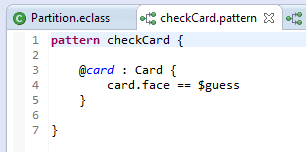
\includegraphics[width=0.5\textwidth]{eclipse_checkPattern}
  \caption{One rule for \texttt{checkCard}}
  \label{fig:checkPattern}
\end{center}
\end{figure} 

\item[$\blacktriangleright$] Lets develop the \texttt{promoteCard} pattern first. It requires three rules, or object variables - the card, the current
partition, and the partition to promote the card must proceed to. Your workspace should resemble Fig.~\ref{fig:promoteCardPattern}.

\begin{figure}[htbp]
\begin{center}
  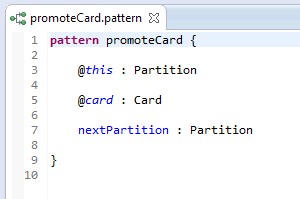
\includegraphics[width=0.5\textwidth]{eclipse_promoteCardPattern}
  \caption{Promoting a card}
  \label{fig:promoteCardPattern}
\end{center}
\end{figure} 

\item[$\blacktriangleright$] Given that \texttt{this} is bound while \texttt{next} is a free variable, we need to establish the reference between this and the
partition, so that the card will move to the correct place. Create a simple reference from \texttt{next} to its target \texttt{nextPartition}. Your file should
now resemble Fig.~\ref{fig:promoteThisRule}.

\begin{figure}[htbp]
\begin{center}
  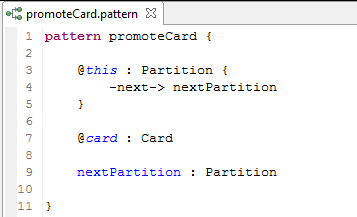
\includegraphics[width=0.5\textwidth]{eclipse_promoteCardThisRule}
  \caption{The \texttt{@this} object variable}
  \label{fig:promoteThisRule}
\end{center}
\end{figure} 

\item[$\blacktriangleright$] Finally, lets create and delete \texttt{cardContainer} references in \texttt{card}. Make a simple destruction reference to
\texttt{this}, and a simple creation reference to \texttt{nextPartition}.\footnote{There are several different ways you could have implemented this movement, such as having a
creation reference in \texttt{nextPartition}} Your pattern is now complete, and should resemble Fig.~\ref{fig:completedPromote}.

\begin{figure}[htbp]
\begin{center}
  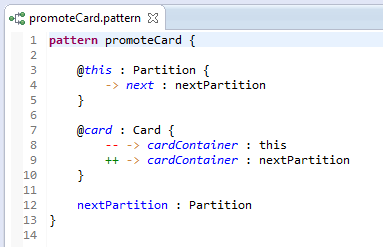
\includegraphics[width=0.6\textwidth]{eclipse_promoteCardCompleted}
  \caption{The finished \texttt{promoteCard} pattern}
  \label{fig:completedPromote}
\end{center}
\end{figure} 

\item[$\blacktriangleright$] Compare the differences between the \texttt{promoteCard} and \texttt{penalizeCard} concepts. They both do the exact same thing,
except the destination partition is slightly different. Knowing this, try to complete \texttt{penalizeCard} entirely on your own.

\item[$\blacktriangleright$] Your workspace should now resemble Fig.~\ref{fig:completedPatterns}.

\begin{figure}[htbp]
\begin{center}
  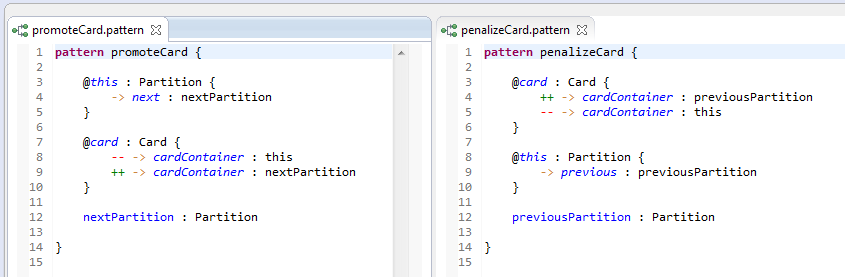
\includegraphics[width=\textwidth]{eclipse_movementPatternsCompleted}
  \caption{The finished movement patterns}
  \label{fig:completedPatterns}
\end{center}
\end{figure}

\item[$\blacktriangleright$] Did you notice that the order of the \texttt{this} and \texttt{card} object variables were reversed in the second pattern? In the
end, it doesn't matter when objects are created, or references are changed in the pattern. Everything just needs to be established in the correct place once
you build your metamodel.

\item[$\blacktriangleright$] The last thing we need to do is complete the control flow. We have specified the assertion and movements, but we haven't
returned any results. If the card was promoted, the guess was successful or \texttt{true}. If it was penalized, the guess was \texttt{false}. Edit
\texttt{partition.check} to reflect this. Your workspace should then resemble Fig.\ref{fig:finalMethod}.

\begin{figure}[htbp]
\begin{center}
  \includegraphics[width=0.7\textwidth]{eclipse_checkMethodFinal}
  \caption{Completed control flow for \texttt{check}}
  \label{fig:finalMethod}
\end{center}
\end{figure}

\item[$\blacktriangleright$] It's now time to build your metamodel. If everything was done correctly, the build will be successful and you can view the changes
in ``PartitionImpl.Java'' under \texttt{check}. You'll be able to see the if/else construct, as well as the link manipulations.

\item[$\blacktriangleright$] Great job! You have just implemented a new control flow and created two card shift patterns. To see how this SDM is implemented
visually, check out Fig.~\ref{fig:sdm_check_finish} for the control flow, and figures \ref{fig:sdm_check_complete_activity_node} and
\ref{fig:sdm_check_complete_penalize} for the movement patterns, all found in the previous section.

% No link since next appropriate page is the literal next page

\end{itemize}
 